\documentclass[12pt,a4paper]{article}
\usepackage[utf8]{inputenc}
\usepackage[siunitx,american]{circuitikz}
\usepackage{pgfplots}
\usepackage[margin=0.5in]{geometry}
\usepackage{textcomp}
\usepackage[spanish, es-tabla]{babel}
\usepackage{amsmath}
\usepackage{graphicx}
\usepackage[colorinlistoftodos]{todonotes}
\usepackage{amsmath}
\usepackage{tikz}
\usepackage{booktabs}

\usepackage{subcaption}
\usepackage{wrapfig}
\usetikzlibrary{arrows}


\usepackage{parskip}
\usepackage{fancyhdr}
\usepackage{vmargin}
\setmarginsrb{3 cm}{2.5 cm}{3 cm}{2.5 cm}{1 cm}{1.5 cm}{1 cm}{1.5 cm}


\pgfplotsset{compat=1.15}

\begin{document}

\part{Diseño de VCO}
\section{Introducción}
En esta sección se busca diseñar e implementar un VCO (\textit{Voltage Controlled Oscilator}) con un rango de trabajo de $0V - 5V$ y que genere una señal senoidal en un rango de $1kHz$ a $10kHz$.

\section{Introducción teórica}

Muchas aplicaciones requieren tener una frecuencia de salida $f_0$ que se programe automáticamente mediante el control de una tensión $V_I$. Este es el trabajo de un $VCO$, que esta diseñado de modo que devuelve:

\begin{equation}
    f_0 = k V_{IN}
    \label{eq:f0}
\end{equation}

Donde $V_I > 0$ y $k$ es la sensibilidad del $VCO$ con unidades de hertz por volt. 



Los $VCOs$ se pueden dividir en dos grupos:


\textbf{Osciladores armónicos}: la salida del oscilador es senoidal. Estos tipos de osciladores son mas difíciles de implementar pero tienen una mejor estabilidad que el otro tipo de osciladores. También, son llamados osciladores de voltaje lineal. Se pueden implementar con circuitos RC, LC o tanque. En estos tipos de osciladores es importante tener en cuenta el parámetro $THD$ (\textit{total harmonic distortion}) que expresa la pureza de la onda senoidal. Su expresión esta dada por:
    
    \begin{displaymath}
        THD (\%) = 100 \sqrt{D^2_2 + D^2_3 + D^2_4 + ...}
    \end{displaymath}

    Donde $D_k (k=2,3,4,...)$ es el ratio de la amplitud del armónico $k$ del armónico fundamental de la serie de Fourier de la onda dada. 

    
    \textbf{Osciladores de relajación}: la salida del oscilador es del tipo triangular, diente de cierra, pulso o cuadrada. En general, son mas fáciles de implementar que los osciladores armónicos. 
    
    \begin{wrapfigure}{l}{0.35\textwidth}
        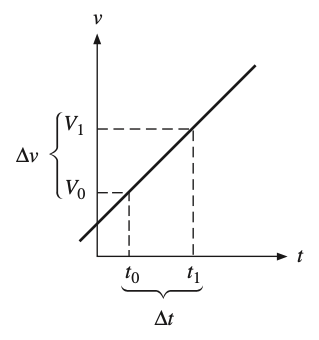
\includegraphics[width=0.9\linewidth]{Resources/lineal_waveform.png}
        \caption{Onda lineal}
        \label{fig:ej3_lineal_waveform}
        \end{wrapfigure}
    
    Para obtener este tipo de salidas se utilizan dispositivos biestables como interruptores, \textit{Schimitt triggers}, compuertas logicas, flip-flops para que rápidamente se pueda cargar y descargar un capacitor.
    

    La descarga y descarga del capacitor es la responsable de dar el tipo de señal de salida. Luego, es de particular interés determinar el $\Delta t$ que le toma al capacitor cargar y descargarse por una determinada cantidad de $\Delta v$. Las formas mas comunes de carga y descarga son la lineal y la exponencial. La primera se da cuando, por el capacitor fluye una corriente constante. Luego, se obtiene una rampa como se ve en la Figura \ref{fig:ej3_lineal_waveform}. Este tipo de función permite estimar  $\Delta t$. Su expresión es:
	\begin{equation}
        \Delta t = \frac{C}{I} \Delta v
        \label{eq:delta_t}
    \end{equation} 

\section{Diseño}

Si bien el objetivo es obtener un $VCO$ cuya salida es una señal senoidal, no se realiza un oscilador armónico sino que se utiliza un oscilador de relajación. Se propone diseñar un oscilador de relajación que devuelva una señal triangular y luego hacer una conversión de dicha triangular a senoidal. En primer lugar se diseña un $VCO$ triangular y luego se diseña con convertor de señal triangular a senoidal. 

\subsection{VCO triangular}


\begin{figure}[h!]                                                       
    \centering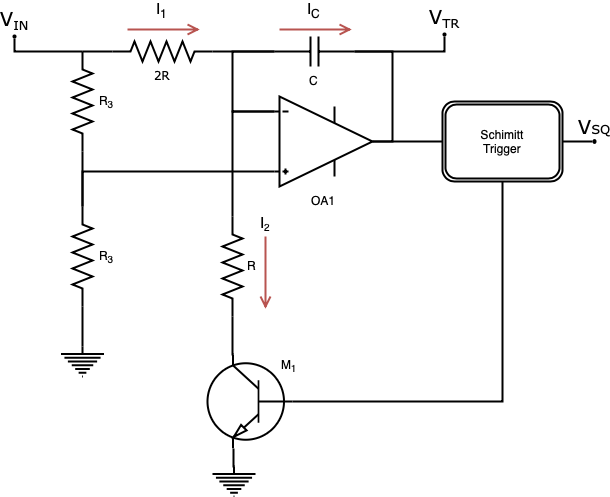
\includegraphics[width=0.6\textwidth]{Resources/circuito_propuesto_1.png}
    \caption{Circuito propuesto VCO}
    \label{fig:VCO_circuito_propuesto_1}
    \end{figure}


Se propone el circuito de la Figura \ref{fig:VCO_circuito_propuesto_1}. Como se puede ver el mismo cuenta con un \textit{Schimitt trigger} como se anticipo en la sección anterior. El amplidicador operacional $OA_1$ es un conversor tension-corriente que fuerza al capacitor $C$ conducir linealmente y proporsional a la tension de entrada $V_{in}$. Se debe tener en mente que, como el capacitor se debe cargar y descargar, la corriente que circula por el capacitor $I_C$ se debe alternar entre polaridades opuestas. 

Antes de comenzar con la explicación del circuito, nótese que, la tensión en ambas terminales de $OA_1$ tienen la misma tensión (se considera al amplificador operacional como ideal) $\frac{V_{IN}}{2}$. Esto surge del divisor resistivo que forman ambas $R_3$. Ademas, se puede calcular la corriente que fluye por $2R$ que es:

\begin{displaymath}
    I_1 = \frac{V_{IN} - \frac{V_{IN}}{2}}{2R} = \frac{V_{IN}}{4R}
\end{displaymath}

Nótese que, $I_C$ es:

\begin{displaymath}
    I_C = I_1 - I_2
\end{displaymath}

Para explicar el funcionamiento del circuito primero se asume que que $V_{SQ}$ comienza en $0V$. Esto implica que el transistor $M_1$ esta apagado por lo que toda la corriente $I_1$ fluye en $C$ ($I_2 = 0A$). Luego, $I_C = I_1$. Al fluir desde la terminal inversora de $OA_1$ hacia la salida de $OA_1$, el capacitor se descarga. Al descargarse, genera una rampa descendiente llevando a $V_{TR} = 0V$. 

Por otro lado, cuando $V_{TR} = 0V$ el tigger \textit{Schimitt} cambia de modo que, $V_{SQ} = 10V$. Esto hace que $M_1$ se encienda poniendo en corto a $R$. Esto implica que $I_2 = \frac{\frac{V_{IN}}{2}}{R} = 2 I_1$. En consecuencia, $I_C = -I_1$. Tomando este sentido, la corriente $I_C$ fluye desde la salida de $OA_1$ hacia la terminal no inversora del mismo, cargando al capacitor y formando una rampa ascendente que lleva a $V_{TR} = 10V$.  

Se puede ver claramente como la corriente del capacitor cambia de sentido formando una señal triangular. A lo largo de todo el ciclo, $I_C$ tiene la expresión:

\begin{equation}
    I_C = \pm \frac{V_{IN}}{4R}
    \label{eq:ic}
\end{equation}




Cuando $V_{TR}$ llega a $10V$ el tigger vuelve a poner a $V_{SQ}$ en $0V$, apagando a $M_1$ y comenzando nuevamente el ciclo (oscila). Resta calcular la frecuencia de oscilación $f_0$. Teniendo en cuenta (\ref{eq:delta_t}) y (\ref{eq:ic}):


\begin{displaymath} \Delta t = \frac{C}{I_C} \Delta V_C = \frac{T}{2} \end{displaymath}
\begin{displaymath} f_0 = \frac{1}{T} \end{displaymath}
\begin{displaymath} \Delta V_C = V_{TH} - V_{TL} \end{displaymath}

\begin{equation}
    f_0 = \frac{V_{IN}}{8RC (V_{TH} - V_{TL})}
    \label{eq:f0_vco}
\end{equation}














\end{document}